% !TEX root = ../YourName-Dissertation.tex
\chapter{Numerical Examples}
\section{Scalar Advection Diffusion Problem}
%%
Here we will look at the scalar valued advection diffusion problem. Let  $\Omega=[0,1]\times[0,1]$. Recall that the scalar valued advection diffusion BVP looks as follows:
%%
\begin{alignat}{2}
    \label{eq: sad}
    \Div{(\bv{a} u - \mu\Grad{u})}-f &= 0 \quad & &\text{in $\Omega$,}
    \\
    \label{eq: sad bound}
    u &= 0 \quad & &\text{on $\partial\Omega$}.
\end{alignat}
%%
The \ac{VMM} yields the following weak formulation: 
\begin{align}
    \label{eq: sad vmm coarse}
    (\tilde{u},\nabla\cdot(\bv{a} u)) + (\nabla\tilde{u},\mu\nabla u) - (\tilde{u}, f) + (\bv{a}\cdot\nabla\tilde{u} + \nabla\cdot(\mu\nabla\tilde{u}),\tau r) &= 0
    \\
    \label{eq: sad vmm fine}
    (\tau,\nabla\cdot(\bv{a} u')) + (\nabla\tau,\mu\nabla u') + (\tau,r) &= 0
\end{align}
where the residual $r$ is given by 
\begin{equation}
    r = \nabla\cdot(\bv{a} u) - \nabla\cdot(\mu\nabla u) - f.
\end{equation}
Equation~\eqref{eq: sad vmm coarse} is the coarse scale problem from the \ac{VMM} and Eq.~\eqref{eq: sad vmm fine} is the fine scale problem for $\tau$ from the \ac{VMM}~\cite{masud2004multiscale}.  We solve Eq.~\eqref{eq: sad vmm fine} first for to find a solution for $\tau$ and then use that solution to solve for the concentration $u$.
%%
Using the ``Weak Form PDE'' interface of \comsol (see~\cite{comsol5.3}) we implemented the numerical solution to the problem specified in Eqs.~\eqref{eq: sad} and~\eqref{eq: sad bound}. We use bubble functions for the fine scale problem and Lagrange quadratic elements for the coarse scale problem. For the convergence study, the method of manufactured solutions is used~\cite{salari2000-MMS}. Our manufactured solution $u$ is the following:
\begin{align}
    \label{eq: sad msu}
    u = \sin\Big(\frac{2\pi(x+y)}{L}\Big).
\end{align}
%%
\begin{figure}
    \centering
    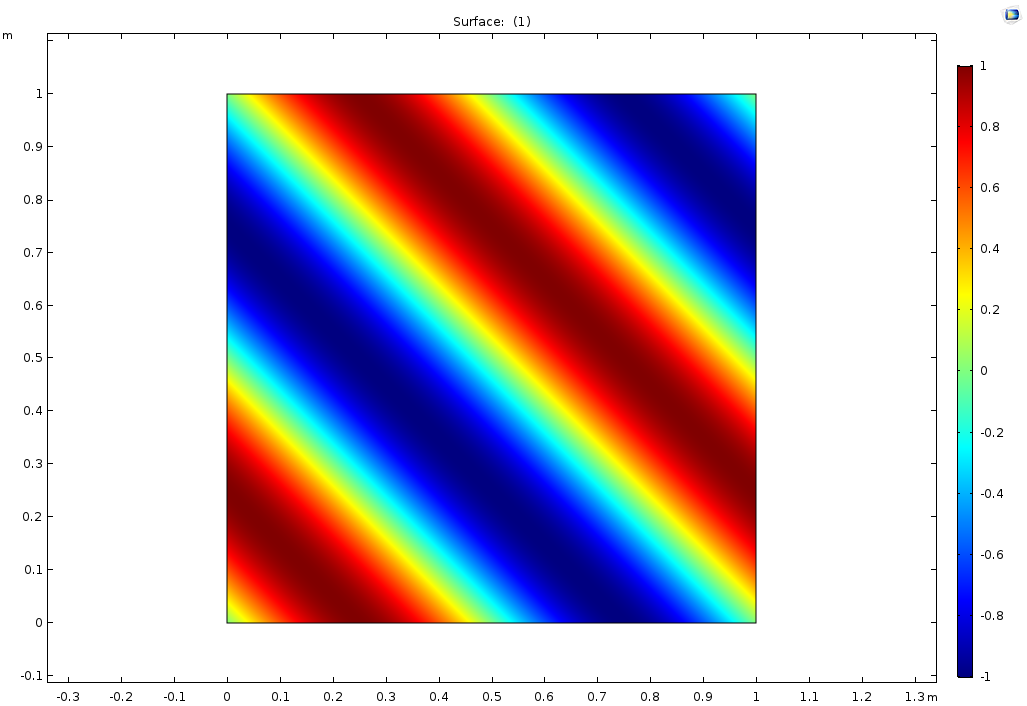
\includegraphics[scale=.5]{Chapter-3/Figures/tauex-MSu.png}
    \caption{Manufactured solution $u$}
    \label{fig:sad msu}
\end{figure}
%%
Then we let $e_u$ be the error of the concentration. From Fig.~\ref{fig:sad conv} we can see that that rates of convergence are comparable to the theoretical convergence rates, that is,
\begin{align}
    ||e_u||_{L^2} = \mathcal{O}(h^3),\\ ||e_v||_{H^1} = \mathcal{O}(h^2).
\end{align}
\begin{figure}
    \centering
    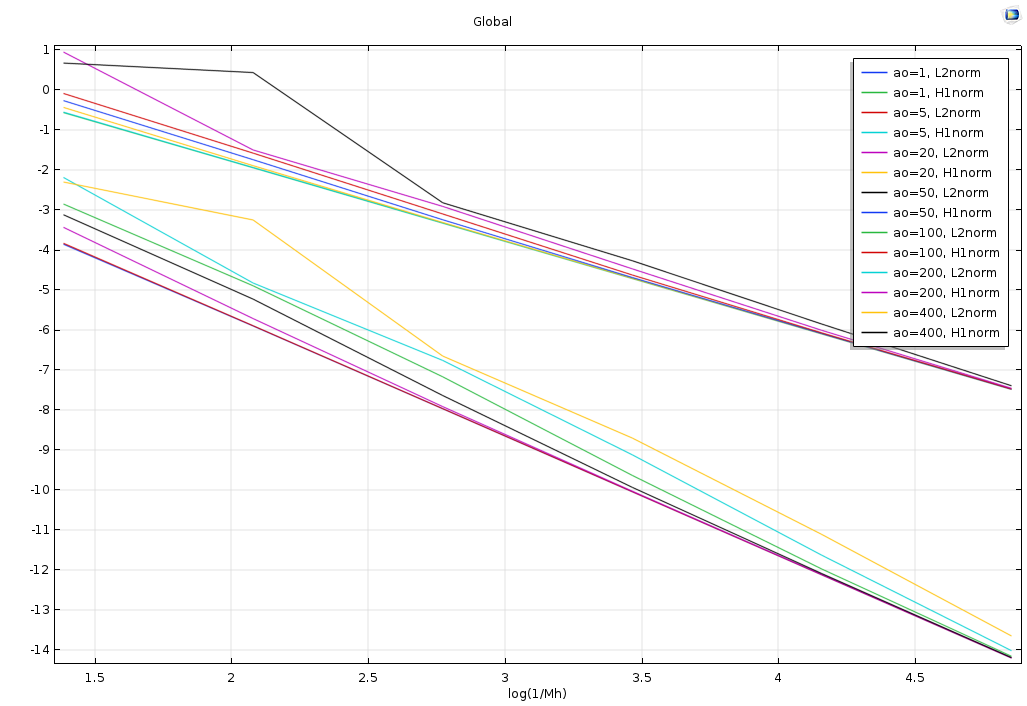
\includegraphics[scale=.5]{Chapter-3/Figures/tauex-conv.png}
    \caption{Convergence rates for $L^2$ and $H^1$ norms for $u$}
    \label{fig:sad conv}
\end{figure}
%%
\section{Navier-Stokes Problem}
In this section we will examine several variations on the Navier-Stokes problem. We will start with a convergence study of the \ac{VMM} stabilized Navier-Stokes problem. Then we will consider two benchmark cases, the steady lid cavity problem and a channel with a cylindrical obstruction. Due to the fact that a solution can be found for these types of problems given enough mesh refinement and time, the meshes used will be relatively coarse in order to test the stabilization effects of the \ac{VMM}.
%%
\subsection{Convergence Study}
Let the domain $\Omega=[0,1]\times[0,1]$. The BVP for the Navier-Stokes problem is as follows:
\begin{alignat}{2}
    \label{eq: NS main eq}
    \rho(\partial_t \bv{v} + \bv{v}\cdot\nabla\bv{v})-\nabla\cdot(p\tensor{I}+2\mu\nabla_{sym} \bv{v})-\bv{b} &= 0 \quad & &\text{ in $\Omega$}
    \\
    \label{eq: NS divv ex}
    \nabla\cdot \bv{v} &= 0 \quad & &\text{ in $\Omega$}
    \\
    \label{eq: NS v boundary}
    \bv{v} &= \bv{v_g} \quad & &\text{ on $\partial\Omega$}.
\end{alignat}
%%
After we put the above BVP, Eqs.~\eqref{eq: NS main eq} though~\eqref{eq: NS v boundary}, through the \ac{VMM} we are left with the following stabilized weak formulation:
\begin{align}
    \label{eq: NS fine scale}
    (\tensor{\tilde{\tau}},(\nabla\tensor{\tau})\bar{\bv{v}}) + (\nabla_{sym} \tilde{\tensor{\tau}},\frac{2}{Re}\nabla_{sym} \tensor{\tau})-(\tensor{\tau},\tensor{I}) &= 0
    \\
    \label{eq: NS coarse scale}
    \begin{split}
        (\tilde{\bv{v}},\bv{v}\cdot\nabla\bv{v}-\bv{b}) + (\nabla\tilde{\bv{v}},-p\tensor{I}+\frac{2}{Re}\nabla_{sym}\bv{v}) +  (\tilde{\bv{v}}\cdot\nabla\tilde{\bv{v}}+\tilde{\bv{v}}(\nabla\cdot\bv{v})+\\\frac{2}{Re}\nabla\cdot(\nabla\tilde{\bv{v}}) + \nabla q,\tensor{\tau}) &= 0
    \end{split}
\end{align}
%%
Eq.~\eqref{eq: NS coarse scale} gives the coarse scale problem that results from the \ac{VMM} and Eq.~\eqref{eq: NS fine scale} is the fine scale problem for $\tau$ from the \ac{VMM} \cite{masud2006multiscale}.
\subsection{Lid Cavity Problem}
The lid cavity problem \cite{masud2009variational} is a problem often used for benchmark testing. In this section we present the steady \ac{VMM} stabilized lid cavity problem. The ``Weak Form PDE'' interface in \comsol was again used to implement the numerical solution. The domain for this study is a unit square with one corner at the origin, \textit{i.e.} $\Omega =[0,1]\times[0,1]$. The domain is discretized into uniform mesh of 1600 elements, where the  A pointwise constraint of zero is applied to the pressure in one corner of the domain. A velocity in the x-direction is applied to the top edge of the domain. 
%%
\subsection{Flow Through a Channel}